
\chapter{Anforderungsanalyse}

\section{Anforderungen laut Regelwerk}
Um am „Carolo-Cup“ Teilnehmen zu können ist ein regelkonformes Fahrzeug notig, darum wird nun ein Auszug aus den Anforderungen an das Auto kurz aufgelistet und ausgewertet.
Alle Anforderungen können im Regelwerk des „Carolo-Cup“ nachgelesen werden \cite{website-carolo-cup-regelwerk}


\subsection{Fahrzeugantrieb und Energieversorgung}
Laut Regelwerk sind alle Teams zur Verwendung eines elektrischen Antriebs verpflichtet.
Die Anzahl der angetriebenen Räder ist nicht vorgeschrieben.
Des weiteren muss das Auto durch Akkus mit Strom versorgt werden.
Die Übertragung von Daten ist während der Dauer der Disziplinen nicht gestattet

\subsection{Fahrzeugantrieb und Energieversorgung}
Es ist eine Zweiradlenkung der Vorderachse vorzusehen. Die übrige Gestaltung des Fahrwerks bleibt den Teams überlassen. Als
technische Ausprägung ist ausschließlich die Achsschenkellenkung zugelassen.

\subsection{RC-Modus}
In Notsituationen muss es möglich sein das Fahrzeug mit Hilfe einer Funkfernbedienung anzuhalten und manuell zu steuern. Eine solche Notsituation tritt ein, wenn
das Auto seine Aufgabe aufgrund eines Fahrfehlers oder anderem Fehlverhalten nicht mehr autonom fortführen kann.
Der RC-Modus muss per Fernbedienung eingeschaltet und ausgeschaltet werden, bei Aktivierung des RC-Modus muss das Fahrzeug unverzüglich angehalten werden.
Während des Wettbewerbs darf die Geschwindigkeit des Autos $0,3\frac{m}{s}$ nicht überschreiten.
Da das 2,4-GHz Band bereits durch die Vorort genutzte Kameratechnik belegt ist können diese Frequenzen nicht für den RC-Modus genutzt werden.
Der RC-Modus muss durch eine blaue Leuchte an der höchsten stelle des Fahrzeuges angezeigt werden, welche mit einer Frequenz von 1-Hz blinkt.

\subsection{Signalleuchten}
Durch die Anlehnung des Wettbewerbes an den realen Straßenverkehr muss das Auto über alle in echten Auto vorhandene Signalleuchten besitzen. 
Dazu gehören 3 rote Bremslichter am Heck des Autos sowie jeweils 2 gelbe Blinker Rechts und Links am Fahrzeug.  Die Blinkfrequenz der Blinker muss
1-Hz betragen.

\section{Auswertung des Regelwerks}
Da ein elektrischer Antrieb vorgesehen ist, muss die nötige Elektronik zur Steuerung des Motors in die Platine integriert werden.
Die Lenkung des Autos kann von einen einfachen Servomotor vorgenommen werden. 
Damit das Auto die im RC-Modus nötigen Funksignale auswerten kann, muss ein Empfänger integriert werden. Dieser wird jedoch über USB zur Verfügung gestellt und ist deswegen nicht Teil dieser Arbeit.
Des weiteren muss das Auto mit den nötigen Signalleuchten ausgestattet sein, dazu gehören Blinker rechts und links jeweils vorne und hinten.
Sowie 3 Bremsleuchten an der Rückseite und eine weitere Leuchte welche din RC-Modus anzeigt. Der Vollständigkeit halber kommt hier noch die
Frontbeleuchtung hinzu


\section{Andere Anforderungen}
\subsection{Anforderungen durch Bewertungskriterien}
Abseits des Regelwerkes ergeben sich weitere Anforderungen durch die Bewertungskriterien des Wettbewerbes. Dabei handelt es sich um nichtfunktionale Anforderungen.
So muss das Team während der statischen Disziplinen ihr Gesamtkonzept präsentieren. Schwerpunkte dabei sind, Hardware und Software Architektur sowie Energiebedarf und 
Herstellungskosten \cite{website-carolo-cup-regelwerk}. Daraus entstehen weitere Anforderungen: Energieeffizienz und Herstellungskosten. \\

Woraus sich Energieeffizienz und Herstellungskosten als Anforderungen ergeben.

\subsection{externe Anforderungen}
Folgende Anforderungen werden durch das Team an die Platine gestellt.
\begin{itemize}
 \item Integration einer Inertialsensorik (Sparkfun SEN-10724)
 \item Anschlüsse für bis zu 6 Infarotsensoren vom Typ Sharp GP2D
 \item Integration einer Odometrie
 \item Stromversorgung eines ``Pandaboard ES'' 
\end{itemize}

\section{Zusammenfassung}

Zusammengefasst werden folgende Komponenten in der Platine benötigt:

\begin{itemize}
 \item nötige Elektonik zur Motoransteuerung (vor und Rückwärts)
 \item Anschluss und Steuerung für einen Servomotor
 \item Anschlusse und Steuerung für die nötige Beleuchtung
 \item Anschlüsse für die Sharp GP2D Sensorn
 \item Integration des Sparkfun Inertialsensors
 \item Leistungsfähige Stromversorgung
 \item Odometrie
\end{itemize}



\todo{


  Vorgehen: Was war seit anfang an vorhanden...,\\
 - warum wurde alter motortreiber (4A) im Prototyp verwendent?\\
 - aus vorhandennen komponenten wurde .. gebaut..
 - folgendes musste verbessert werden!
 

}

\todo{


 - Konzept überabrbeiten...
  - Vierquadrantensteller ins konzept--> wie soll es umgesetzt werden.
  - Anforderungsanalyse vor das Konzept
  - 
 

}



% Das Team setzt ein Fahrzeug vom Typ TT-01 Type E des Herstellers Tamiya ein. Dabei handelst es sich um ein modellbau Auto. Dieses Modell wird bereits mit
% Motor und Fahrtenregler ausgeliefertund entspricht den vorgaben im Regelwerk. Da am Lehrstuhl bereits größere Mengen an LiPo-Akkus mit einer Nennspannung von 14,4V vorhanden sind, sollen diese verwendent
% werden. Da der dem Auto beiliegende Fahrtenregler nicht für eine derart hohe Spannung ausgelegt ist, ist hier ein Ersatz notwendig. 
% 

% 
% Im folgenden wird geklärt wie das Fahrzeug vom Team geplant und umgestetzt wird. Das Fahrzeug basiert auf einem Modellbauauto vom Typ TT-01 Type E des Herstellers Tamiya. 
% Das Auto besteht dabei aus folgenden Komponenten: einem Elektromotor zur Fortbewegung, einem Servomotor zur Lenkung, einer Kamera welche die Fahrbahn aufzeichnet, einer Recheneinheit welche
% die Bildverabreitung und Regelung des Fahrzeuges übernimmt und einer Treiberplatine. 
% 
% 
% \subsection{Die Treiberplatine}
% Die Treiberplatine hat hat die Aufgabe die Sensorik und Aktorik mit der Recheneinheit zu verbinden. Zusätzlich befinden sich auf ihr eine Spannungsversorgung, ein Motortrieber und
% diverste Anschlüsse fürdie Sensorik. Die Platine wurde in 2 Versionen erstellt. Da für die 1. Platinenversion eine Ansteuerung durch GPIO-Pins des Pandaboards geplant war. Durch den
% späteren Wechsel zum Intel NUC, welcher nicht über GPIO-Pins verfügt, musste eine überarbeite Version der Platine entwickelt werden. Welche ien einfachen Anschluss an den NUC gewährleistet.
% Die 
% 
% Die Treiberplatine wurde 
% 
% In Abbildung [\ref{fig:platine_rv3}] ist das Board der überarbeiteten Platinenversion zu sehen.
% 
% \begin{figure}[H]
% \centering
% 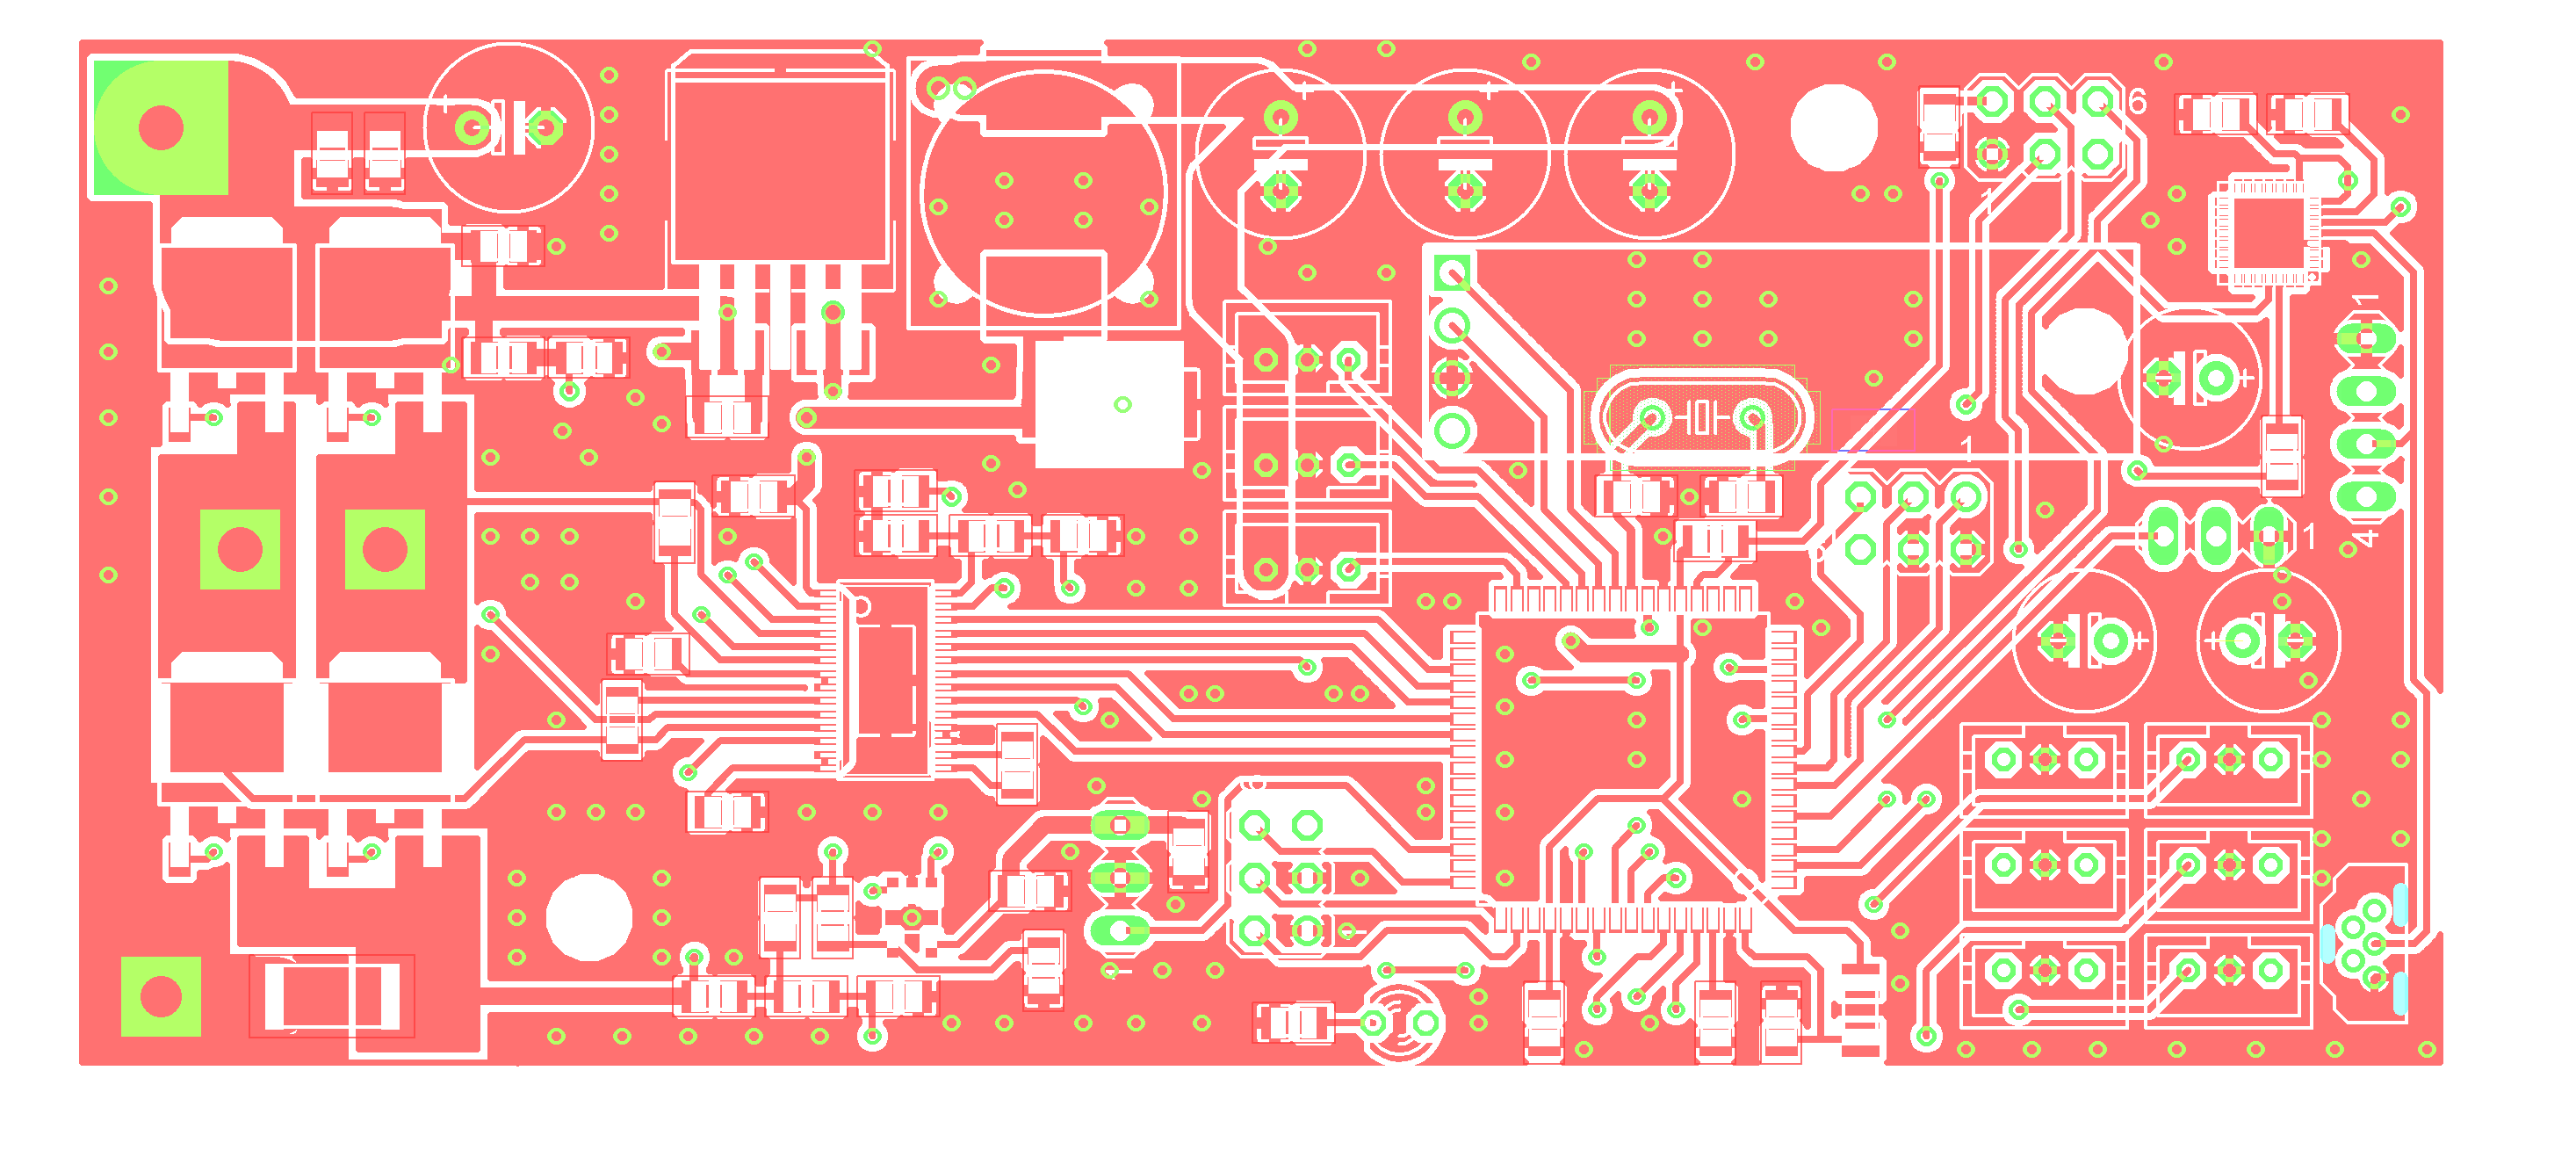
\includegraphics[width=.8\textwidth]{platine_rv3.png}\\
% \caption{Korrigierte Platinenversion}
% \label{fig:platine_rv3}
% \end{figure}
% 
% 
% 
% 
% 
% 
% 
% 












